\section{Embodied AI}

一路走来我们的工具是逐渐齐全的, 任务是逐渐丰富的. 但是这些任务都是基于被动的数据输入,
还没有接触过机器自主的与环境交互, 现在希望能具备在 pyhsical world 进行交互的能力.

\subsection{Embodied AI}

\textbf{具身智能是什么?}

这个词语出现非常久了, 但是中国在23年左右才开始提.
Turing 提到, 人工智能有两种和人竞争的方法, 第一种是使用搜索等方法, 解决类似下棋的问题; 
第二种就是具身智能, 使用传感器, 涵盖了知识传递的过程.

经典智能, 只具有人类大脑的能力, 计算能力; 但是人在大脑之外还具有交互能力, 这就是 embodied AI.

具身智能相比基于数据的智能近两年才火起来, 也是因为具身智能不像网络上有那么多数据.

\textbf{\\Embodiment 是什么?}

Embodiment 就允许了你去探索环境, 和环境交互, 得到经验. 
这个过程既给了你探索的能力, 也对你作出了限制, 车是不能飞的.

有人讲, Embodied AI 是通向 AGI 的必经之路, 道理就是如果一个 agent 没有interaction 的能力,
就不能认为它是 AGI 的.

比如 Hand-Eye Coordination任务, 人类也不是天生具有的, 需要后天学习, 甚至很多
Hand-Eye Coordination 任务现在也不会, 比如 Juggling ball.

\textbf{\\你觉得大自然中有没有 AGI? }

思考的智能可能不具备, 但是 embodied 智能是很强的.

从上述讨论中抽象出来一个高于 Perception-only 的 paradigm, 
也就是 Perception-Action Loop\footnote{强化学习-like}.

人类的学习大部分就是 Perception-Action Loop, 只有少部分, 比如学习考试, 是 supervised learning.
Perception-Action Loop 是我们现在模型中很欠缺的.

\textbf{\\Scaling law是不是通向AGI的唯一方法?}

For sure answer is no. 

Data driven 是有用的, 但是纯互联网数据是不够的, 现在的
ChatGPT-4o 等大模型基本上已经穷尽了互联网数据(但是还没有将算力使用枯竭), 
每周再爬取几十 Terabytes 数据就是现在唯一的数据来源了,
或许还有一些侵犯版权的数据. 并且互联网上的数据只占每人每天的数据的一小部分,相信你不会把自己
的所有行为都放在互联网上.

但是现在还有大量的数据还没有利用, 就是Perception-Action Loop的数据, 
这样的数据暂时还不存在很多, 比如自动驾驶数据可能有一些,但是只能在特定环境下使用.

一般来讲我们相信 Perception-Action Loop 是下一个阶段的 AGI 的重要数据源泉.

\textbf{\\Now and Future for Embodied Al}

1. Industrial Robots and Autonomous Driving for now.

但是不好说 Industrial Robots 是一个 AI. 因为这些机器人是在一个非常特定的环境下工作的, 
所有运动路径都是 hard code 的.

另外一个就是 Autonomous Driving, 比如 Tesla 准备在2024年8月在美国进行 robotaxi 服务
测试, 使用FSD(Full Self-Driving)技术, 他们宣称这是一个 end2end 的 imitation learning.
这就是一个典型的 embodied AI, 并且是 data-driven, 也符合 Perception-Action Loop的paradigm.

但是显然这样的数据 DOF 还是太低了, 控制还是比较简单, 但是需要安全度很高, 
99\%或者99.9\%也不算绝对安全,
至少需要像人一样开车上万公里才出现一次失误才足够.

对于Tesla这样的技术, 如果一个季度没创死人, 就算是 revolutioanry.

2. Home robots for future.

制造一个像人一样的通用机器人. 但是这样的机器人需要具备很多能力, 比如抓取、操作、导航等等.

老师上课提到了转笔, 这可能是在说2023年的这篇论文\cite{ma2023eureka}, 这篇论文采用
LLM driven的reward fine-tuning, 在物理仿真中实现了非常灵巧的转笔任务.

同时 locomotion 这也是一个非常难的任务, 这样的下肢任务是落后于上肢运动的, 容错率也很低.

老师认为 embodied AI 可以支持AI再发展20年.

\subsection{Object Grasping}

prehensible: 可理解的, 可抓取的.

\textbf{\\不同的抓取稳定性}

Non-force closure: 靠力保持稳定.

Force closure: 靠力保持稳定, 能容忍任意一个方向的加速度.

Form closure: 靠形状保持稳定, 任意一个方向的速度都不会让物体脱离.

\textbf{\\怎么做呢?}

主流方法是使用 detection 方法, 跟RCNN一样把所有抓取方法都检测一遍, 
可以像object detection一样算recall和precision.

但是需要数据集, 多少数据够呢?很多, 所以需要synthesize很多数据.

这篇论文\cite{fang2020graspnet}在88个物体上使用Force closure的constraint上
synthesize 了十亿个数据,结果是可以泛化到所有物体上.

为什么使用点云? 只在意形状, 不在意颜色.

泛化性来源于什么? 点云中的局部相似性, 也就是说, 一个点云可以抓取的局部形状是可以泛化到其他物体上的.

\textbf{\\Cons?}

透明物体或者说不是漫反射的很难抓取.

可以通过synthetic data训练模型来解决这个问题.

\textbf{\\一个发现}

Synthesize大量数据集同时进行domain randomization, scale很大之后,就可以泛化到真实世界了.

曾经 Google 在真实世界使用7台机械臂+RL在RGB模态下训练Grasping, 
用一年达到了87\%的准确率,但是不能泛化到其他环境, 抓取台一旦改变就不work了.
问题就在于RGB模态对于环境是不具有泛化性的.

\subsection{Object Manipulation}

老师上课提到的OpenAI拧魔方是这篇工作\cite{openai2019solving}, 
试图在物理仿真中进行策略学习然后泛化到真实世界.

其中最重要的idea是使用 Automatic Domain Randomization (ADR),让物理仿真中的
Domain Randomization自动化改变, 而不是人类手动改变环境参数, 从而使得模型可以泛化到
更加复杂的环境中.

作为一个魔方爱好者, 其实这样的结果距离真正的 One-handed Rubik's Cube
还有较大差距, 但是对于这样一个 Training from scratch 的工作, 可以实现这样的效果已经是非常了不起的了.

但是更重要的事情是只学这一个是远远不够的, 这样的policy是不具有到其它任务上泛化性的.

\textbf{Dexterous Hand}

手的自由度是非常高的, 一只手可能就有22到25个自由度, 赋予了人极高的自由度, 但是学习难度也非常高.

Shadow Hand 100w 人民币. Dexterous hand 是达到人类灵巧度的希望.

\textbf{Related work}

Learning Category-Level Generalizable Object Manipulation Policy: 基于强化学习的抓取.

GAPartNet: 基于监督学习的抓取.

DexGraspNet: 大型抓取数据集.

\subsection{Locomotion and Navigation}

四个轮子已经解决, 四条腿比较难, 两条腿基本上还没解决.

传统的locomotion 机器人不使用视觉, 但是现在希望结合视觉信息.

\textbf{Nevigation Tasks}

Point Goal: Go 5m south, 3m west relative to start

Image Goal: Go where the photo was taken.

Object Goal: Go to the red chair.

\textbf{Nevigation Methods}

Classical Modular Navigation: Mapping, Planning, Execution

End-to-end Reinforcement Learning: imitation learning (behavior cloning), RL

\textbf{Related work}

考试不要求相关论文

Online 3D Recon. and Navi. (CVPR 2023): RL

Mobile Manipulation (ICRA 2024): RL, loco-manipulation

\subsection{Embodied Multimodal Large Model}

真正的 AGI 的可能形态.

\begin{figure}[H]
    \centering
    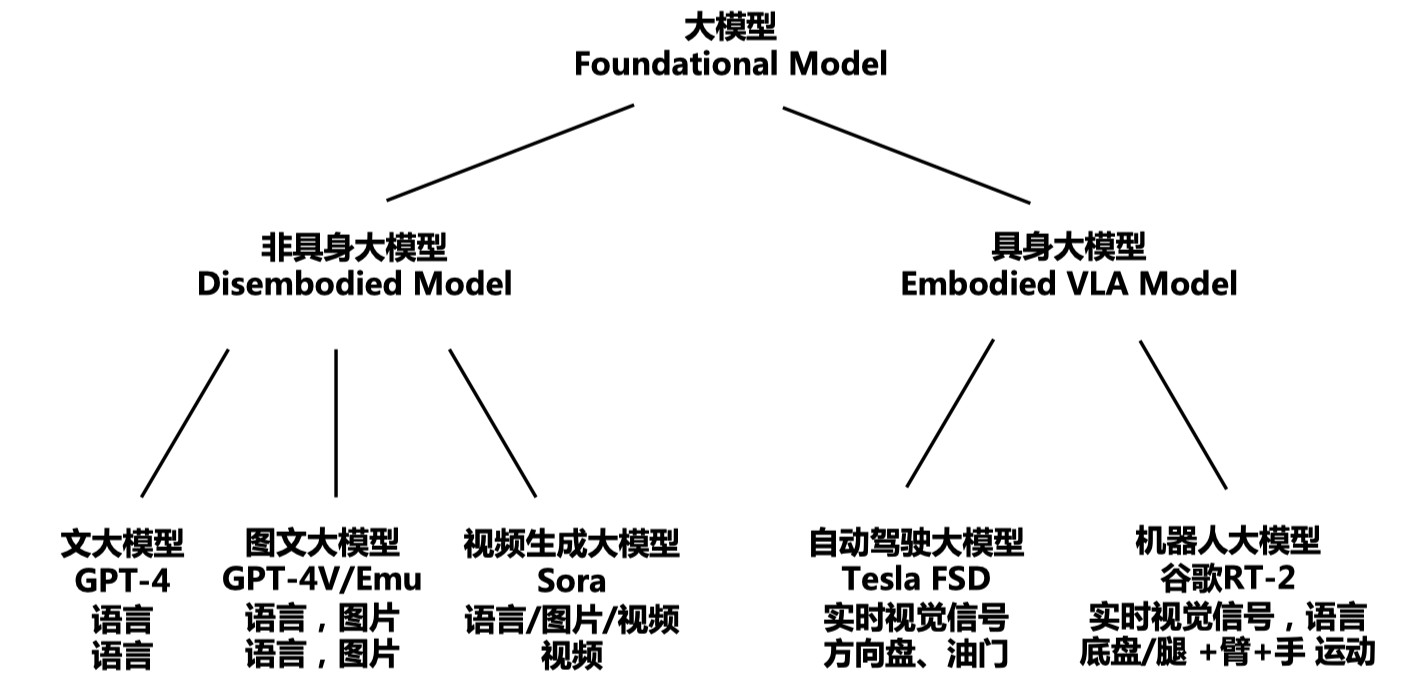
\includegraphics[width=0.8\textwidth]{figures/Embodied_Multimodal_Large_Model.png}
    \caption{Multimodal Large Model}
\end{figure}

RT-1: 采集13万条数据,以97\% 的成功率抓取一个厨房里面的物体, 做了一年半, 使用imitation learning学习的.

RT-2: 问题也在于泛化性不好, 数据也不够.

估计使用上万亿个小时的视频才可以做到真正的泛化 embodied AI.

老师认为使用合成数据是好的.
